\documentclass[.../main.tex]{subfiles}

\begin{document}

    This segment of research aims to achieve a deeper understanding
    of the strategy evolution of agents following a Q-Learning
    approach. This allows for guarantees to be placed on the behaviour
    of such agents, in particular the conditions under which the game
    will converge to a stable equilibrium.

    It has long been established that, upon lifting the strong
    assumptions made by traditional game theory (such as the
    rationality of agents and complete information), that player
    strategies can result in much more complex behaviour than
    convergence to a Nash Equilibrium (NE). In fact, this is even true
    on what would commonly be regarded as 'simple' games such as
    tic-tac-toe and prisoner's dilemma \cite{Galla2011,
      Sato2002}. These behaviours include: convergence to a unique
    equilibrium (though not always to an NE), convergence to one of
    multiple equilibria, limit cycles and chaos. These behaviours are
    shown in Figure \ref{fig::DynamicalBehaviours}. Of these, the most
    preferable is, of course, convergence to a unique equilibrium,
    although it is still possible to study systems with multiple
    equilibria or limit cycles \cite{Strogatz2000}. However, it would
    be difficult to control systems whose dynamics are governed by
    chaos (though research into controlling chaos is ongoing and rife
    with opportunity \cite{Fradkov2009}) and so MARL techniques should
    avoid this. It would, therefore, be a useful endeavour to
    determine the conditions under which these sorts of behaviours
    arise.

    \begin{figure}[h]
        \centering
        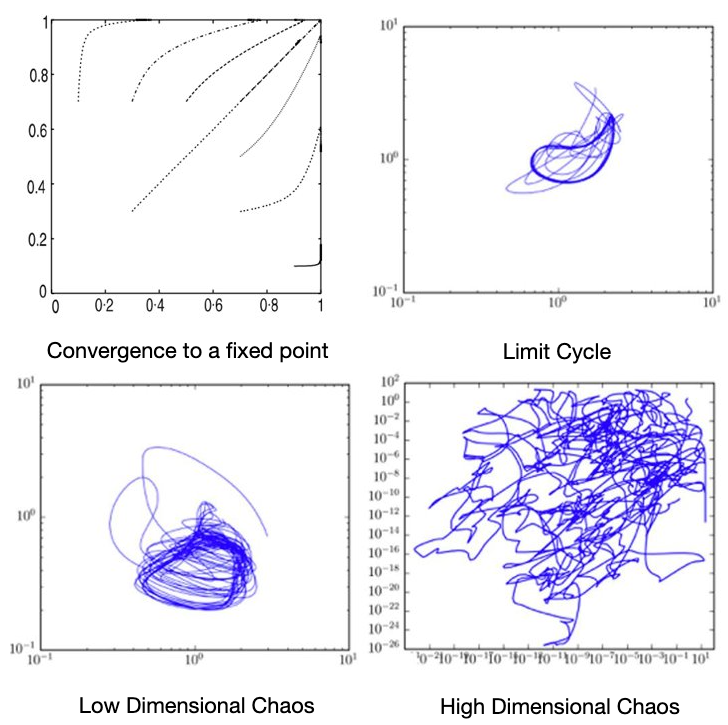
\includegraphics[width=1.1\textwidth]{Figures/DynamicalBehaviours}
        \caption{ \label{fig::DynamicalBehaviours} Different types of dynamical behaviour
       displayed
        by learning agents. a) Figure drawn from \cite{Tuyls2006AnGames}.
        Convergence
        to a unique fixed point in the upper right corner (1, 1). This fixed point is unique, in
        that all trajectories, regardless of initialisation, will converge to this point. b) Limit Cycle, the trajectories converge to cyclic behaviour c,
        d) Chaotic behaviour, here small deviatons in the initial conditions can grow
        exponentially. b-d drawn from \cite{Sanders2018}}
    \end{figure}

    The behaviour of a system may be studied given a model of its
    dynamics. It is through this process that a wide array of physical
    systems, from harmonic pendulums to geophysical fluids, can be
    understood. A growing body of research aims to understand
    multi-agent reinforcement learning through the lens of its
    dynamics. In this light, Tuyls et al. \cite{Tuyls2006AnGames} were
    able to derive a model of the strategy evolution of agents
    learning through iterated games.  Through this, they were able to
    arrive at the following model of Multi-Agent Q-Learning

    \begin{subequations}
    \label{eqn::EOM}
        \begin{equation}
            \frac{\dot{x}(t)}{x(t)} = \alpha \tau (\sum_{j} a_{ij} y_j - \sum_{i j} x_i a_{ij} y_j)
            + \alpha \sum_j x_j ln(\frac{x_j}{x_i}) 
        \end{equation}
        \begin{equation}
            \frac{\dot{y}(t)}{y(t)} = \alpha \tau (\sum_{j} b_{ij} x_j - \sum_{i j} y_i b_{ij} x_j)
            + \alpha \sum_j y_j ln(\frac{y_j}{y_i}).
        \end{equation}
    \end{subequations}

    Here, $\alpha$ and $\tau$ are the parameters of the agent; Sanders et al. refer to these as the
    memory and intensity of choice parameters respectively. Agent 1 takes action $i$ with probability
    $x_i$ while Agent 2 takes action $j$ with probability $y_j$. If these actions are taken, the agents
    receive payoff $a_{ij}$ and $b_{ji}$ respectively. With these equations, it is possible to
    predict the expected behaviour of Q-Learning agents, as shown in Figure 
    \ref{fig::TuylsExperiments}.

    \begin{figure}[h]
        \centering
        \begin{subfigure}[b]{0.9 \textwidth}
            \centering
            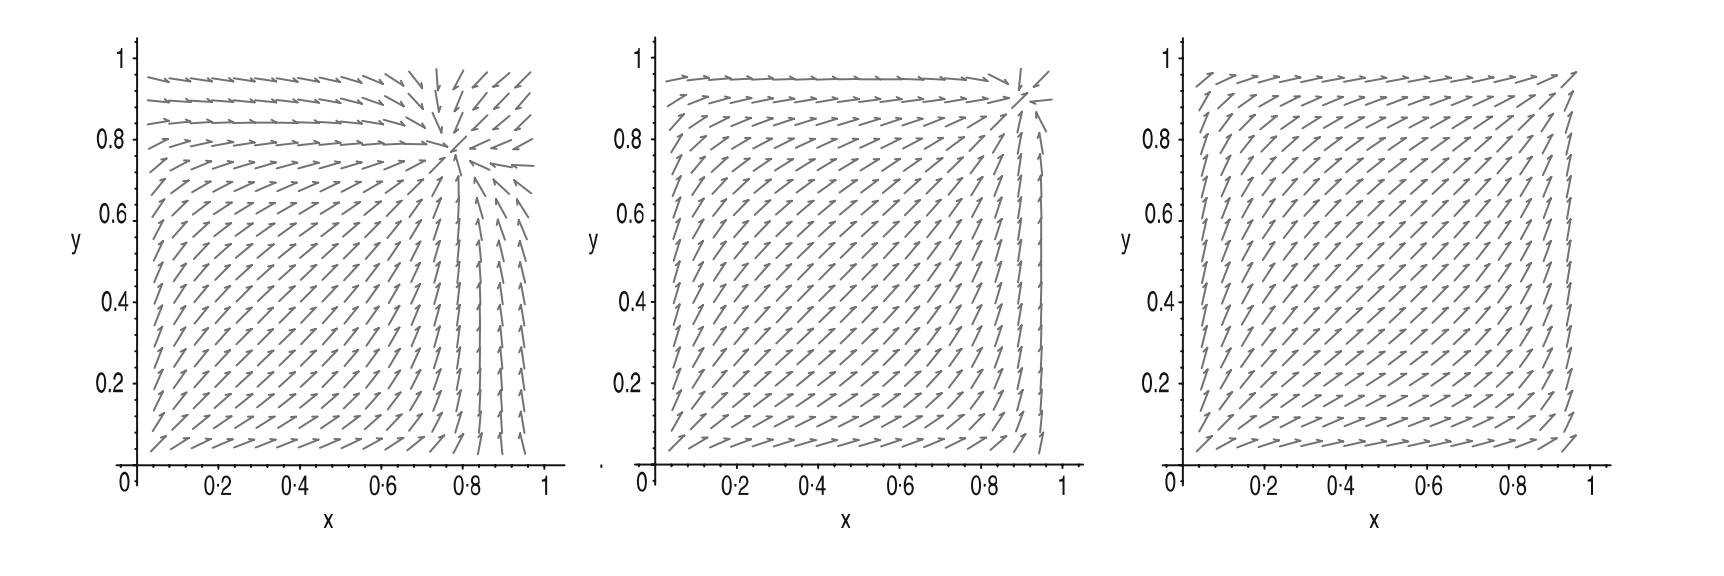
\includegraphics[width=0.75 \textwidth]{Figures/Dynamics}
            \caption{}
        \end{subfigure}
        
        \begin{subfigure}[b]{0.9 \textwidth}
            \centering
            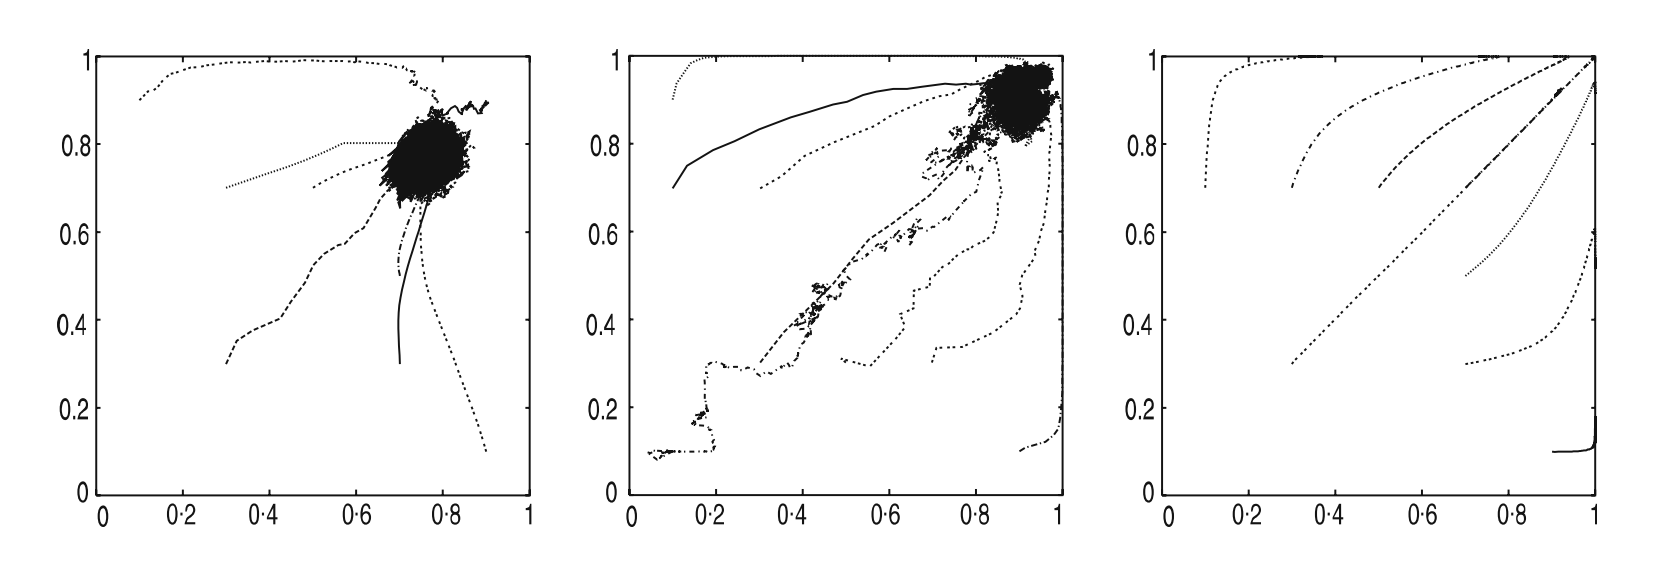
\includegraphics[width=0.7 \textwidth]{Figures/Q-Learners}
            \caption{}
        \end{subfigure}

        \caption{ \label{fig::TuylsExperiments} Figures taken from \cite{Tuyls2006AnGames} a) Phase
        plot showing the expected behaviour of Q-Learning agents trained by iterating the
        Prisoner's Dilemma game as predicted by (\ref{eqn::EOM}). From left to right, the agents
        have parameter $\tau = 1, 2, 10$. b) Corresponding trajectories of Q-Learning agents with
        randomised initial conditions displayed through numerical simulation. It is clear that the
        trajectories in b) follow the predictions in a), after stochasticity is accounted for. }
    \end{figure}    

    It is clear, both from (\ref{eqn::EOM}) and Figure \ref{fig::TuylsExperiments}, that the long-term strategy selection of
    these agents is determined by the parameters $\alpha, \tau$ and the payoffs $a_{ij}, b_{ij}$. We
    then pose the question: how do these elements influence the types of behaviours seen during
    learning on an iterated game? In other words, under what parameter selections are we likely to
    see convergence to unique equilibria, multiple equilibria, limit cycles or chaos?

    With this in mind, the intention of this area of study is to consider the analysis presented in
    works such as \cite{Sanders2018} and \cite{Galla2011}. Here, the authors examine the
    Experience Weighted Attraction (EWA) algorithm, which is regarded as a strong model for the
    learning behaviour of human players in a game \cite{Camerer2009}. The authors are able to
    determine the regions of parameter space in which complex behaviour,
    including cycles and chaos, predominantly occur and those in which a given game converges to a
    stable equilibrium. Figure \ref{fig::GallaPredictions} reproduces the graphs shown in \cite{Sanders2018} which
    illustrates the successful derivation of a `phase line', across which learning shifts from
    convergent to chaotic.

    \begin{figure}[h]
        \centering
        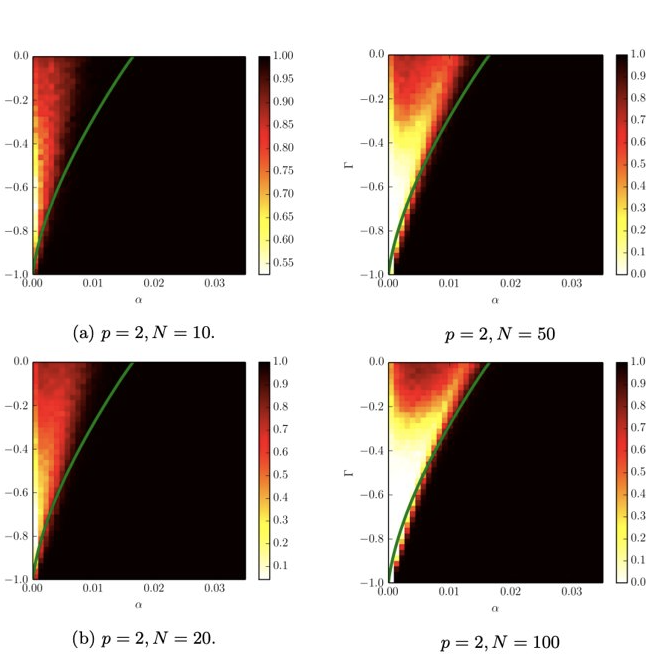
\includegraphics[width=0.6\textwidth]{Figures/GallaPredictions}
        \caption{ \label{fig::GallaPredictions} Results as produced in the supplementary material
        of Sanders et al \cite{Sanders2018}. Here, $p$ is the number of players, $N$ is the number
        of actions, $\Gamma$ represents the competitiveness of the game (-1 represents zero-sum, 1
        represents shared rewards) and $\alpha$ is the memory parameter of the agent as before.
        Here $\tau$ is held constant at 0.05 (though it is referred to as $\beta$ in the paper).
        The black region represents where games converged to a fixed point through all simulations,
        whilst the hotter regions represent the more complex dynamics - red shows the presence of
        limit cycles and white regions signal the onset of chaos. The green line is a theoretical
        estimation for the phase line which separates the convergent dynamics from complex.}
    \end{figure}

    We propose to bridge the analysis presented by Sanders
    et al. and Galla et al. towards games learnt using MARL, particularly Q-Learning with
    Boltzmann exploration as considered by Tuyls et al. This would allow for a characterisation of
    the expected resultant behaviour under given parameters for a particular game. The vision for
    this is to provide guarantees on the stability of a finite set of agents within a swarm, such as
    leaders in a flock. Without this, it would be impossible to ensure the stability of a swarm in
    which intelligent, social interactions must be accounted for. In addition, this analysis
    would allow for a characterisation of the conditions under which MARL algorithms may
    feasibly be applied, thereby supporting the ability of researchers and engineers to choose their
    payoff matrices and parameters accordingly.

\section{Summary of Research}

    In this chapter, we summarise and present the research and results
    which have been obtained thus far. These tackle the problems
    described thus far in this chapter. We summarise the
    derivation of a stability phase line as presented in Sanders et
    al. \cite{Sanders2018} as well as the numerical simulations
    performed to verify these results. These details of the derivation are provided in Appendix 
    \ref{app::ResearchSummary}. The steps to be completed
    subseqent to this study are then given. Note that the results in the section form the basis of a
    tentative submission to AAAI 2021. 

    \section{Convergence and Chaos in Q-Learning Agents} \label{sec::Chaos_in_Q-Learning}

    We begin by considering the evolution of learning with agents who
    follow a Q-Learning approach.  Specifically, we look at
    characterising the stability of agents learning strategies. This
    technique is carried out by Sanders et al. \cite{Sanders2018}, in
    which the authors characterise the strategy evolution of agents
    who learn using an 'Experience Weighted Attraction' (EWA)
    algorithm, which has been shown to be a strong representation of how
    people learn in games \cite{Camerer1999, Camerer2003}. The authors are able to determine the
    regions of parameter space in which learning is likely to converge
    towards stable equilibria, as opposed to complex behaviours
    (such as limit cycles or chaotic dynamics). The aim of this study
    is to format these techniques for the study of computational
    agents who follow the popular Q-Learning approach
    \cite{Sutton2018,SchwartzMulti-agentApproach}.

    We aim, similarly, to determine the regions of parameter space in
    which the agents are likely to converge to stable equilibria. In
    this way it will be possible to, a priori, determine whether, for
    a particular game, the behaviour is likely to converge and even
    how to choose the agent or game parameters to ensure the
    predicatability of the resulting behaviour. To achieve this, we
    consult the Q-Learning Dynamics proposed by Tuyls et al
    \cite{Tuyls2006AnGames}. In this study, the authors were able to
    derive a continuous time dynamical system describing how agents
    following a Q-Learning approach adjust the probabilities of
    choosing actions as they iteratively play a game. These equations
    are shown in \cite{Tuyls2006AnGames} to accurately model the
    expected behaviour of agents as they iterate a game, and the
    experiments which verified this model are shown in Figures
    \ref{fig::TuylsExperiments}.

    With the accuracy of the continuous time dynamical system
    (\ref{eqn::EOM}) established, we analyse the stability of this
    system in the following section. Note that whilst the derivation
    provided is for the particular case of two agents for the sake of
    brevity, the problem of $p$-player games is equivalent to that of
    two players and so the solutions to the former can (and will) be
    presented.

    \fr{differences/similarities between EWA and Q-learning?}
    
    \subsection{Dynamics of Q-Learning} % (fold)
    \label{sub:dynamics_of_q_learning}
    
    We begin with the popular Q-Learning algorithm in which each agent keeps a record of a `Q-Value'
    for each action, which is its own estimation of the performance of said action. This estimation
    is based on the expected reward that the agent will receive if it were to choose this action. In
    a multi-agent game setting, the reward that an agent receives will be drawn from a payoff
    matrix and will depend on the behaviour of the other players. Taking this into consideration,
    an agent updates their Q-Value of action $i$ with the equation

    \begin{equation}
    \label{eq::Q-Learning}
    Q_{t+1}(a_i) = (1 - \alpha) Q_t(a_i) + \alpha (\sum_j a_{ij} y_{j} + \gamma max_{a_j}Q_t(a_j)).
    \end{equation}

    Here, $\alpha \in [0, 1]$ is a parameter of the agent which is considered the {\em memory} of
    the agent. For low values of $\alpha$, the agent places a higher weight on their pre-existing
    choice for $Q_t(a)$, and so is considered to have a longer memory, whereas for higher values of
    $\alpha$, the agent has a higher propensity to disregard previous estimations in favour of new
    information. Note that the term $\sum_{j} a_{ij} y_j$ denotes the expected reward that the agent
    will receive for selecting action $i$, drawn from its payoff matrix $A$, given the probabilities
    that its opponent chooses any action $j$. At each iteration of the game, our agent selects an
    action to play randomly with probabilities given by

    \begin{equation}
    \label{eq::actionselection}
    x_{i} = \frac{e^{\tau Q_t(a_i)}}{\sum_j e^{\tau Q_t(a_j)}}.
    \end{equation}

    This introductes a new parameter, $\tau \in [0, \infty)$, which is considered the {\em intensity
    of choice} by Sanders et al. \cite{Sanders2018}. When $\tau$ is close to zero, each action $i$
    is played with the same probability, regardless of its Q-value. However, for large values of
    $\tau$, the action with the highest Q-value dominates all others and is played with a large
    probability at each step. The value of $\tau$, then, denotes an agent's propensity to explore
    its strategy space. Note that in this derivation, as in \cite{Tuyls2006AnGames}, the
    action probabilities of one agent are denoted with $x$ and those of its opponent are denoted
    with $y$. The payoffs received by these agents are given by $a_{ij}$ and $b_{ij}$ respectively.

    Tuyls et al. use this Q-Learning formulation to determine the time evolution of $x$ and $y$.
    Given a continuous time approximation of this behaviour, they arrive at the equation 
    \ref{eqn::EOM} which is repeated below for convenience.

     \begin{subequations}
        \begin{equation}
            \frac{\dot{x}(t)}{x(t)} = \alpha \tau (\sum_{j} a_{ij} y_j - \sum_{i j} x_i a_{ij} y_j)
            + \alpha \sum_j x_j ln(\frac{x_j}{x_i}) 
        \end{equation}
        \begin{equation}
            \frac{\dot{y}(t)}{y(t)} = \alpha \tau (\sum_{j} b_{ij} x_j - \sum_{i j} y_i b_{ij} x_j)
            + \alpha \sum_j y_j ln(\frac{y_j}{y_i}).
    \end{equation}
    \end{subequations}

    We now seek to analyse the stability of these dynamics based on the payoff values and agent
    parameters ($\alpha, \tau$).
    % subsection dynamics_of_q_learning (end)

     \subsection{Derivation of stability line} % (fold)
     \label{sub:derivation_of_stability_line}
    

    The dynamics given by Tuyls et al. describe the time evolution of agent
    strategies for a given choice of $a_{ij}, b_{ij}$. However, our goal is to
    analyse the dynamics of any game, regardless of payoff elements. As such,
    we follow the approach of Sanders et al. in deriving the full set of
    'effective dynamics' averaged over all possible realisations of the payoff
    matrices. We consider that these elements are drawn from a Multivariate Gaussian
    such that

    \begin{equation*}
        \begin{split}
            \mathbb{E}[a_{ij}] = \mathbb{E}[b_{ji}] = 0\\
            \mathbb{E}[a_{ij}^2] = \mathbb{E}[b_{ji}^2] = 1\\
            \mathbb{E}[a_{ij} b_{ji}] = \Gamma.
        \end{split}
    \end{equation*}

    where $\Gamma$ is a parameter which defines the `competitiveness' of the game. For a two player
    game, $\Gamma \in [-1, 1]$ where -1 denotes a zero-sum game and 1 denotes a game with positive
    correlation across payoff elements. Taking this average (details given in Appendix 
    \ref{app::ResearchSummary}) yields
%
    \begin{equation}
    \begin{split}
        \dot{x}(t) &= x(t)(\Gamma \alpha^2 \tilde{\tau}^2 \int dt'[G_y(t, t')x(t')] + 
        \tilde{\alpha}
        \rho_x(t) + \alpha \tilde{\tau} \eta_x(t) + \tilde{\alpha} \tau \eta_x(t) \eta_y(t) +
        \sqrt{\Gamma} \tilde{\alpha} \tau \mu_x) \\
        \dot{y}(t) &= y(t)(\Gamma \alpha^2 \tilde{\tau}^2 \int dt'[G_x(t, t')y(t')] + 
        \tilde{\alpha} \rho_y(t) +
        \alpha \tilde{\tau} \eta_y(t) + \tilde{\alpha} \tau \eta_x(t) \eta_y(t)+ 
        \sqrt{\Gamma} \tilde{\alpha} \tau \mu_y), \\
    \end{split}
    \end{equation}

    Here, $G, \rho, \eta, \mu$ are correlation functions, generated due to the averaging process 
    and the notation $\tilde{\cdot}$ denotes a term which has been scaled with respect to $N$ 
    (again, see Appendix \ref{app::ResearchSummary} for method and notation). We now analyse the
    stability of this dynamical system by linearising about a fixed point. This yields the
    requirement that a fixed point $x^*$ satisfy

    \begin{equation}
    0 = x^* \left[\Gamma \alpha^2 \tilde{\tau}^2 x^* \int G_y(t - t') dt' + \tilde{\alpha} \rho_x^*
    + \alpha \tilde{\tau} \eta_x^* + \tilde{\alpha} \tau \eta_x^* \eta_y^* + \sqrt{\Gamma} 
    \tilde{\alpha} \tau \mu_x \right],
    \end{equation}

    and similary for y. The reader should be aware that, for the sake of brevity, only the equations
    for $x$ are presented henceforth as those for $y$ are equivalent.

    The implication here is that the resulting value of $x^*$ can take two
    solutions. However, one of these is $x^* = 0$, which is found to rarely
    occur \cite{Coolen2005} and we do not consider, while the second,
    non-trivial solution contains a term $\sqrt{\Gamma}$, which would yield
    complex values. Such a result, of course, is not possible for a quantity
    denoting probabilities and so it appears that the theory cannot hold for
    $\Gamma < 0$. However, numerical experiments will shed light on the
    likelihood of convergence and the islands of stability in parameter space
    for this region.

    We take the Fourier transform of this system to determine the long term behaviour of the system
    after a disturbance. To neglect all transient behaviour (high frequency disturbances), we
    consider the equation at $\omega = 0$

    \begin{equation} \label{eqn::Transformed}
    \left<[|\mathcal{X}(\omega)|^2 \right> = \left< | \Gamma \alpha \tilde{\tau} \mathcal{V}_x(\omega) + \tilde{\alpha} \tau \eta^*_x \mathcal{V}_y(\omega) + \tilde{\alpha} \tau \eta^*_y \mathcal{V}_x(\omega) + \sqrt{\Gamma} \tilde{\alpha} \tau \Delta(\omega) + \Xi(\omega) |^2 \right> \frac{1}{\left< |\mathcal{A}(\omega, x^*) |^2 \right>}, 
    \end{equation}


    where

    \begin{equation}
        \mathcal{A}(\omega, x^*) = \frac{i \omega}{x^*} - \Gamma \alpha^2 \tilde{\tau}^2 \mathcal{G}_y(\omega)
    \end{equation}

    By
    considering that $\left<|\mathcal{X}(\omega =
    0)|^2
    \right> \geq 0$  we arrive at an expression for a stability line (i.e. the phase transition
    between the
    existence of stable fixed points and unstable behaviour) as the equality (\ref{eqn::Transformed}
    )$>0$.

    % subsection derivation_of_stability_line (end)

    \subsection{Numerical Experiments} % (fold)
    \label{sub:numerical_experiments}
    
    To verify the results of our theory, and to examine the underlying structure of stability and
    chaos in Multi-Agent Q Learning, we perform a series of numerical experiments by varying the
    parameters $\Gamma$ and $\alpha$ whilst keeping $\tau$ fixed. This yields the result shown in
    Figure \ref{fig::NumericalExperiments}. We see from this, and from the further experiments shown
    in Appendix \ref{app::ResearchSummary}, that the stability of the system is highly dependent on
    the value of $\tau$.
    For
    low values, the system converges almost everywhere, whilst increasing $\tau$ to 0.15 decreases
    the probability of convergence significantly.

    \begin{figure}[h]
        \centering
         \begin{subfigure}[b]{0.45 \textwidth}
        \centering
        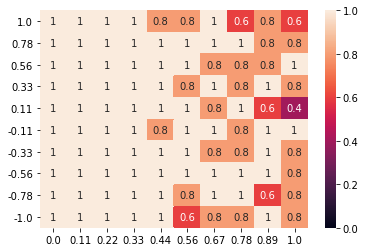
\includegraphics[width = 0.7 \textwidth]{Figures/AlphaRun_tau_005.png}
        \caption{$\tau = 0.05$}
        \end{subfigure}
        \begin{subfigure}[b]{0.45 \textwidth}
        \centering
        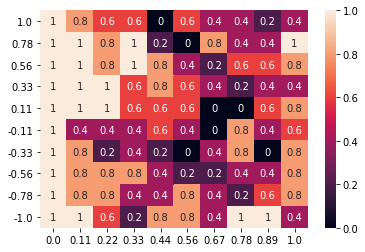
\includegraphics[width = 0.7 \textwidth]{Figures/tau_015.png}
        \caption{$\tau = 0.15$}
        \end{subfigure}

        \caption{$\alpha = 0.1$, $\gamma = 0.1$, $\tau \in [0.1, 10]$, $\Gamma \in [-1, 1]$. Each
        simulation is run for 1 $\times 10^5$ iterations and tested for convergence. The game is
        said to have
        converged based on a tolerance of 1\% difference between action probabilities. For each
        combination of $\tau$, $\Gamma$ the game is played 5 times, each with random payoff matrices
        and initial conditions. The average number of converged games (giving an indication of
        probability of convergence) is shown in each cell of the heatmap. 
        \label{fig::NumericalExperiments}}
    \end{figure}

   To generate the numerical simulations in Figure \ref{fig::NumericalExperiments} we used the
   following procedure.

\begin{enumerate}
    \item Fix the parameters $\alpha$ and $\gamma$. The latter is held fixed at $0.1$ since
    it does not affect the long term behaviour of the system (it does not appear in (
    \ref{eqn::EOM})).
    \item We initialise values of $\Gamma$ and $\tau$. These will be the variables which we sweep
    over.
    \item Generate payoff matrices for both agents by sampling from a multi-variate Gaussian 
    (variables are the payoff elements) with covariance parameterised by $\Gamma$.
    \item Initialise the agents with random initial conditions (i.e. random action probabilities).
    \item Allow the agents to learn over a maximum of $1 \times 10^5$ iterations.
    \item Every 100 iterations, check to see if the action
      probabilities have changed significantly.  If not (i.e., the
      change over the last 100 iterations is less than 1\%) the
      learning process is considered to have converged.
    
    \item This process is repeated 5 times with random payoff matrices generated based on the value
    of $\Gamma$. The probability of convergence is then recorded as $\frac{\text{number of times
    converged}}{5}$.

  \item The values of $\tau$ and $\Gamma$ are then modified and the process is repeated. The
    heatmap shows the probability of convergence for all values of $\tau$ and $\Gamma$ which are
    tested.
\end{enumerate}

    % subsection numerical_experiments (end)

    \subsection*{Future Work} \label{sec::Future Work}

    We are currently running a set of numerical experiments varying over all three parameters
    $\Gamma, \alpha, \tau$ to identify any islands of stability in parameter space. We will then
    plot (\ref{eqn::Transformed}) to verify our results.

    As mentioned, the above system considers only a two player game. This was done with the intention
    of simplifying the notation and reducing the complexity of the experiments. However, the next
    immediate action is to present the equivalent solutions for the case of a general $p$-player
    game.
    
    We then seek to expand this study to a population of agents. For
    this, we will study the stability of the system presented by Leung
    et al \cite{Hu2019} which presents a mean-field model describing
    the evolution of learning of a population of Q-Learning agents who
    play co-operative games against one another. This is discussed further in the subsequent chapter
    on proposed research.

\end{document}
